\documentclass[a4paper]{article}
\usepackage{graphicx}

\begin{document}

\title{Analyzing Unoccupied Setback Effectiveness and Prevalence via K-Means Clustering}
\author{Jay Herron}
\maketitle

\section{Intro}

Reducing energy use in buildings is expensive. Despite advances in fault-detection and diagnostic systems, acheiving building energy savings still requires manual effort to evaluate issues and make the necessary virtual or physical changes to rectify them. Because of this, there is a need for improved prioritization in order to satisfy the biggest opportunities first.

Historically, prioritization has typically taken two paths:
\begin{enumerate}
\item{High level metrics: Industry standard metrics like energy use intensity are used to compare buildings to their peers and grade their efficiency. Unfortunately, these metrics do very little to suggest actions to take for energy reduction within a given building.}
\item{Low level analytics: Analytics identify discrete operational issues which are extremely useful for determining actions to take. However, these rarely output energy savings estimates, and when they do the values are unreliable because system interaction is often complex.}
\end{enumerate}

There is opportunity for a middle layer that improves high level prioritization and provides a clear path to implementation.

This document proposes a set of key performance indicators (KPIs) and an analysis framework to identify and prioritize energy reduction through unoccupied setbacks. Nearly every building can acheive significant energy reductions by basic changes to their unoccupied operation, and these savings are extremely cost-effective. The largest energy savings opportunity in most non-industrial building involves modifying zone air temperatures, minimum discharge air flow setpoints, or lighting based on occupancy. The propsed framework identifies these opportunities.

\section{Approach}

This framework requires whole-building energy use values at hourly frequencies or faster. This data is readily available for 80 of the buildings in the RTEM dataset. Whole-building energy usage is then cleaned by removing meter rollover artifacts, aligning timestamps to a consistent frequency, and interpolating missing values. Next, values are dis-aggregated if they are represented by a monitonically increasing value, and finally they are passed through an outlier filter. After this process, we are left with clear, consistent energy usage data for the whole building.

Next, the cleaned data is split into weekly periods and passed through a k-means clustering algorithm that identifies 2 nodes: a "high-usage" cluster and a "low-usage" cluster. This process provides a mapping between each energy usage reading and whether it belongs in the high or low usage, as well as values for the high and low-usage clusters. We interpret the high-usage period to be the occupied time in a building, and the low-usage period to be the unoccupied time.

From these results, we can compute two meaningful weekly KPIs:
\begin{enumerate}
\item{Unoccupied Turndown Factor: The high-usage value divided by the low-usage value. Scaled from 0 to 1, lower values indicate more effective unoccupied setbacks. Lower is better from an energy reduction standpoint.}
\item{Occupied Duration Factor: The amount of time the building was in a high-usage state, divided by the total time in the KPI period. Scaled from 0 to 1, lower values indicate more prevalent unoccupied setbacks, in terms of time.  Lower is better from an energy reduction standpoint.}
\end{enumerate}

This simple approach offers several distinct advantages. First, the data requirements are extremely low; only a single historical reading for total energy use is required. Of the 230 buildings in the RTEM dataset, 99 have "Electric Consumption" points, making it the 5th most prevalent point behind "Virtual", "Zone Temperature", "Outside Air Temperature", and "Status". Second, it is widely applicable. The analysis process is not impacted by the type of building, the pattern of occupancy throughout the week, or the type of equipment within the building. Since no assumptions are made on the time of occupancy, it functions as well on irregularly occupied buildings (like community centers or theaters) as on regularly occupied buildings (like commerical office buildings or retail). Finally, it delivers actionable results. Even the most primitive control systems offer features for modifying building operation according to occupancy.

\section{Usage}

These KPIs alone do not scale according to energy usage, so they are best used as part of an Energy Use Intensity-based analysis. For example, if comparing buildings within a portfolio, the EUI could be used to determine the worst-performing facilities, and then the KPIs above could be used to determine whether these facilities would benefit from improving the unoccupied operation.

The different KPIs suggest different actions:
\begin{itemize}
\item{A large Unoccupied Turndown Factor suggests that unoccupied operation should be investigated. When unoccupied, minimum discharge airflow setpoints should be going to 0, zone air temperature setpoint deadbands should widen significantly, and lights should be shut off if possible. Also, this KPI suggests that there may be areas that never enter an unoccupied state.}
\item{A large Occupied Duration Factor suggests that occupancy detection systems should be investigated. Of course, unoccupied energy saving measures must conform to each building's unique occupancy patterns. However, if occupancy is based on a schedule, that schedule should be checked to ensure that it matches actual occupancy patterns. If occupancy is detected using a sensor, the sensors should be validated for correct operation.}
\end{itemize}

While a KPI value on a particular building at a particular time is meaningful, KPIs are typically most useful when they are compared between entities or over time. A building with a large KPI value compared to its peers, or with a KPI value that increases over time may provide context on what a "large" KPI value is.

\section{Results}

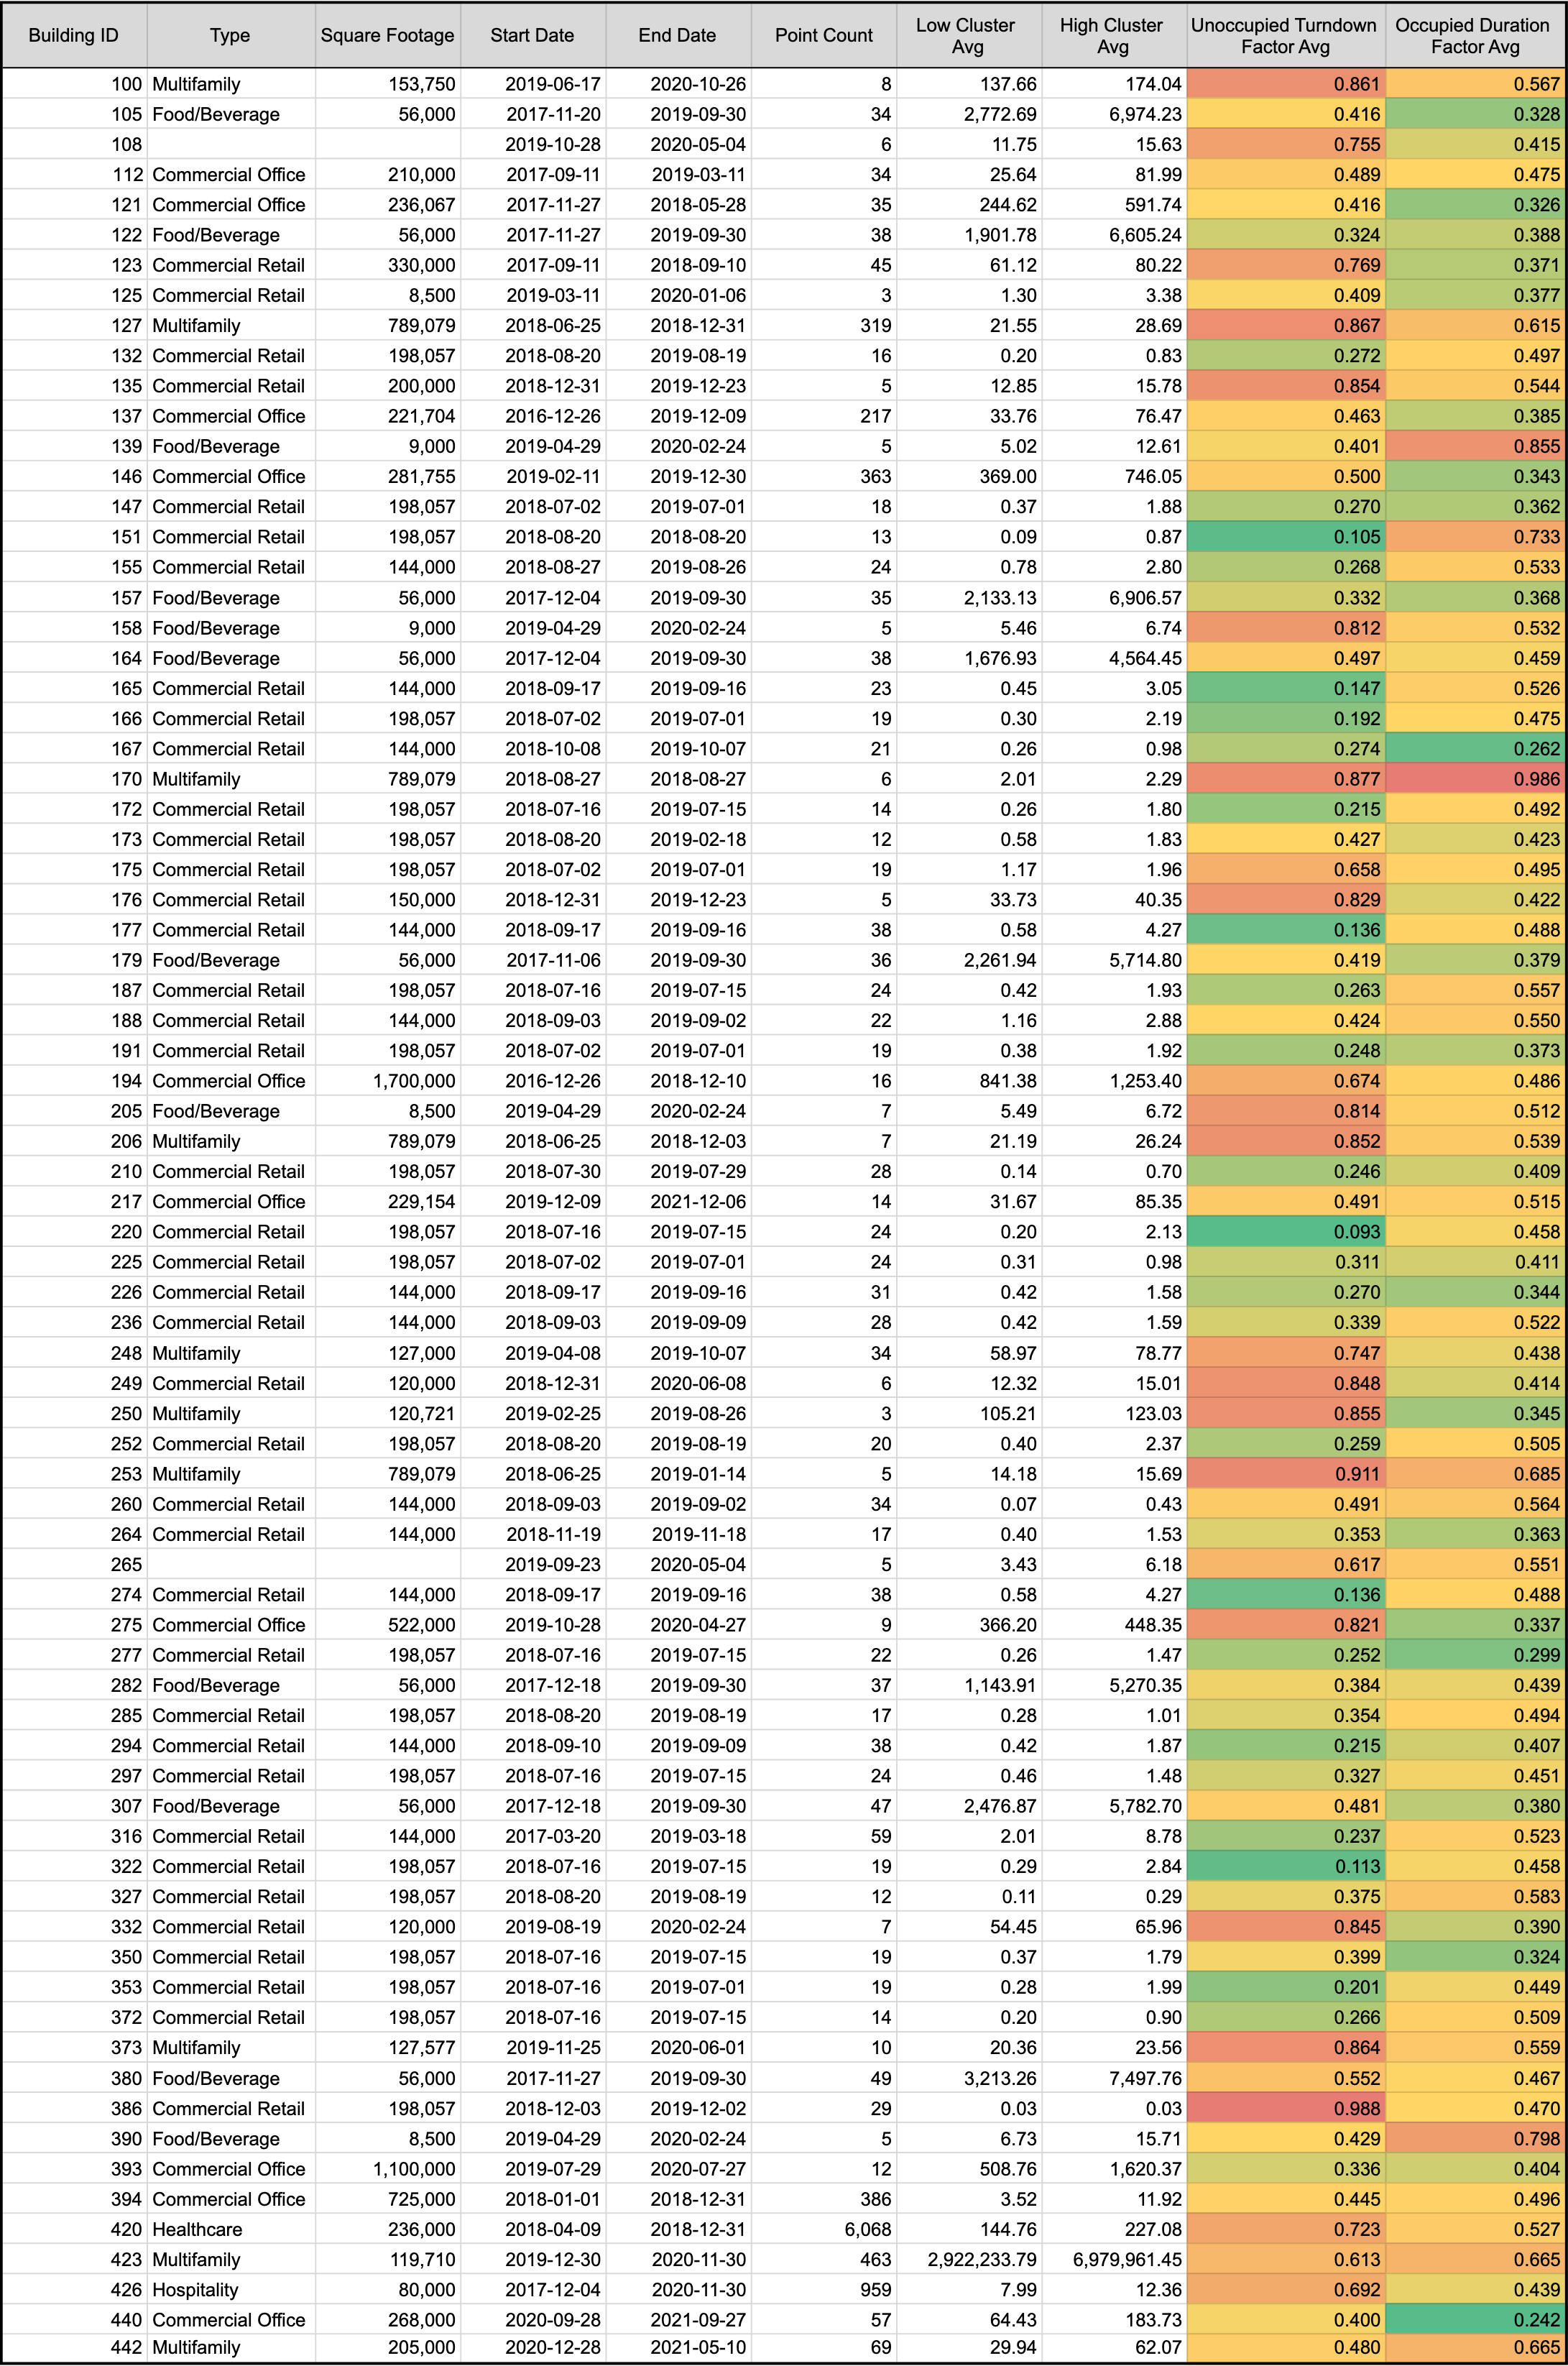
\includegraphics[width=\columnwidth]{./images/KPI_Result_Table.png}

\section{Analysis}

\subsection{Building 188}

Building 188 and Building 165 are similarly sized commercial retail spaces with significantly overlapping datasets and similar occupied usage, but differing values for the unoccupied turndown KPI. Observing the usage over time, we can indeed see a larger usage in Building 188 during unoccupied times.

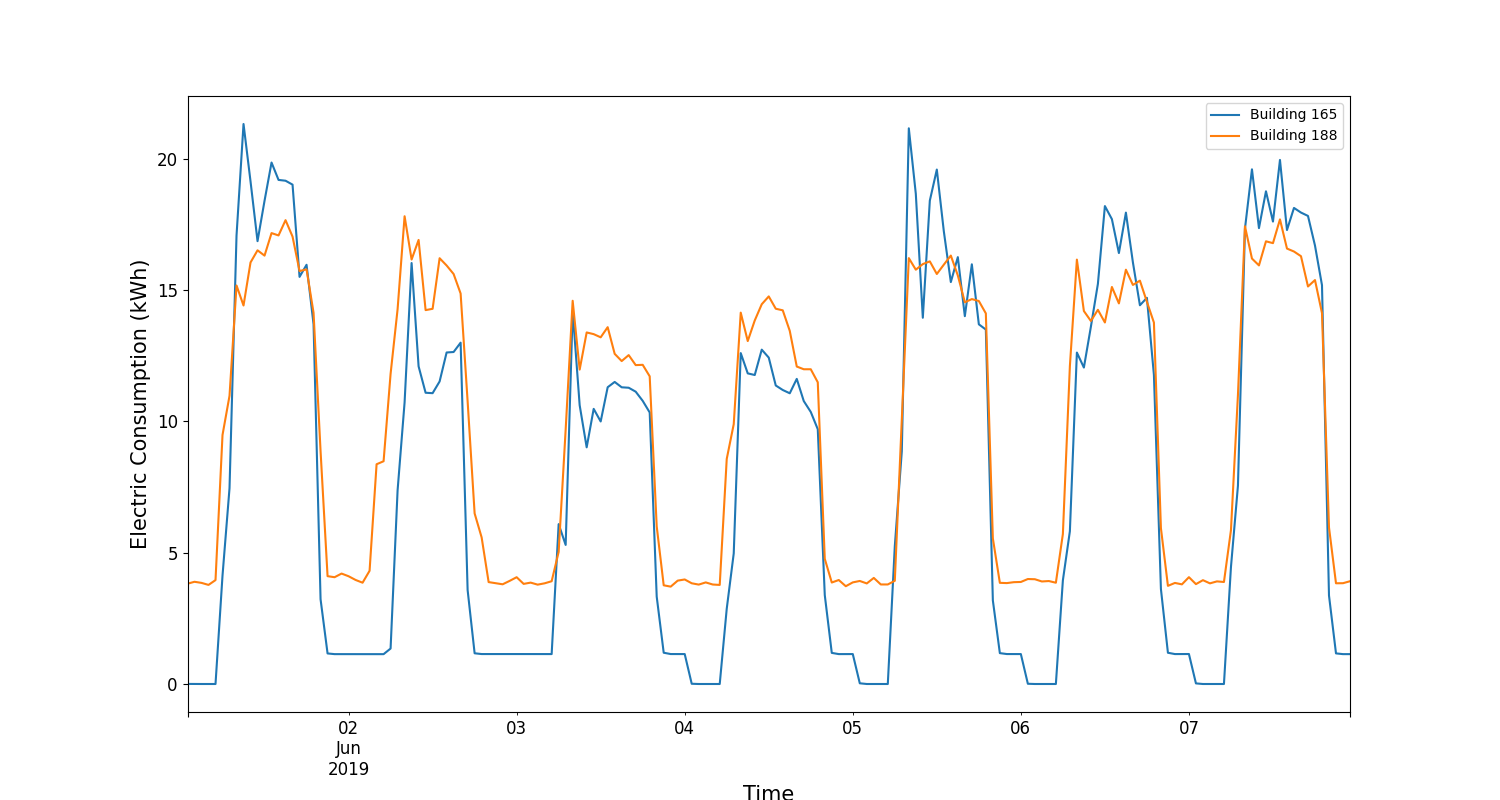
\includegraphics[width=.8\columnwidth]{./images/188v165_Turndown.png}

Investigating the HVAC submetering shows that the nighttime usage in 188 is unrelated to the HVAC equipment.

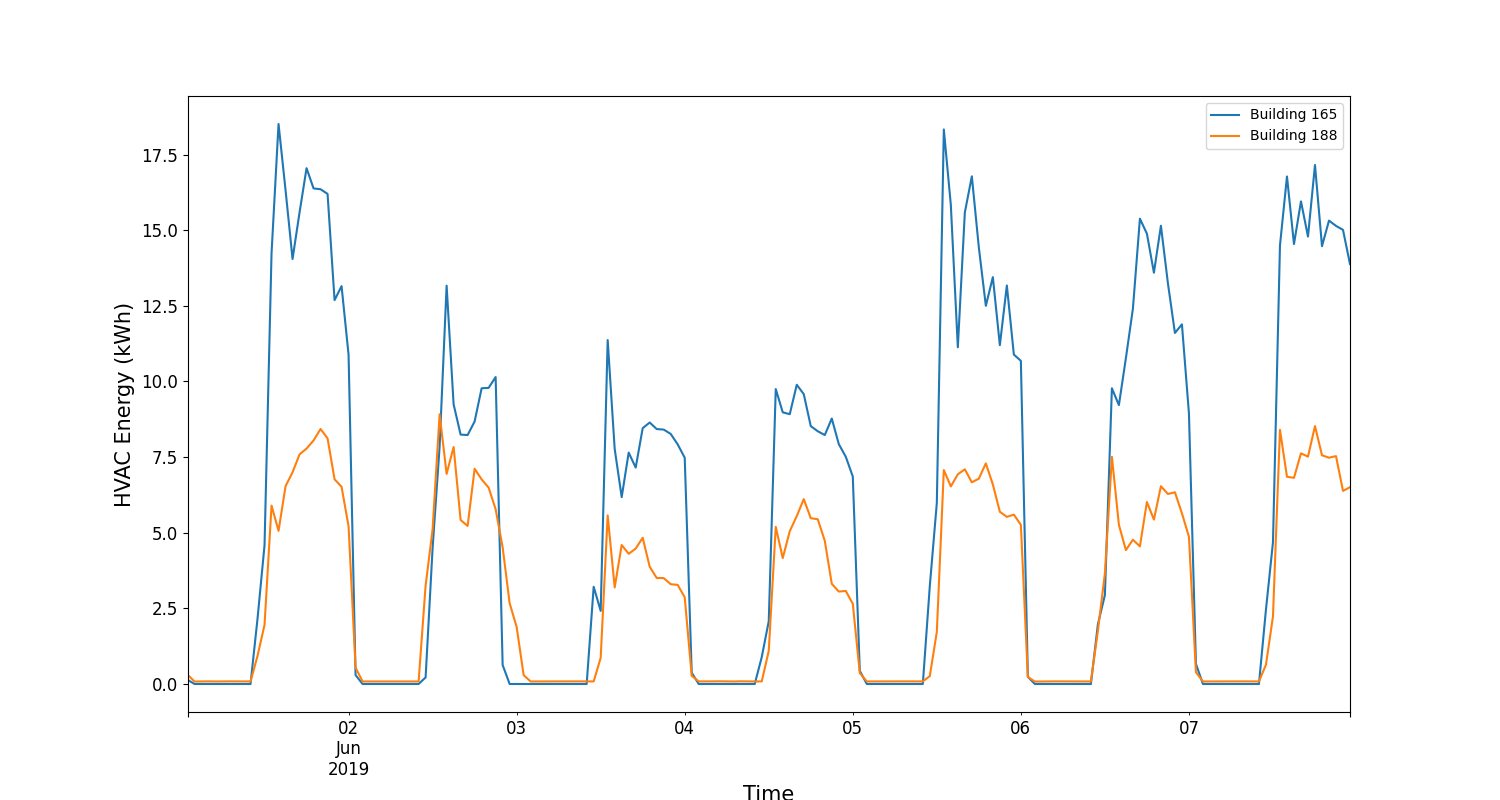
\includegraphics[width=.8\columnwidth]{./images/188v165_Turndown_HVAC.png}

This suggests that the nighttime usage is a result of some unmeasured load, likely lighting or plug loads.

If Building 188 was able to achieve a turndown equivalent to that of 165, the KPIs suggest that it would reduce energy consumption by roughly 11,500 kilowatt-hours per year, which is roughly 16\% of its total yearly energy usage.

\subsection{Building 275}

Building 275 and 393 are both commerical office buildings. 393 has twice as much square footage and its energy needs are much higher. However, with an unoccuiped turndown factor of 0.821, Building 275 has a much flatter profile than 393, whose factor is 0.336.

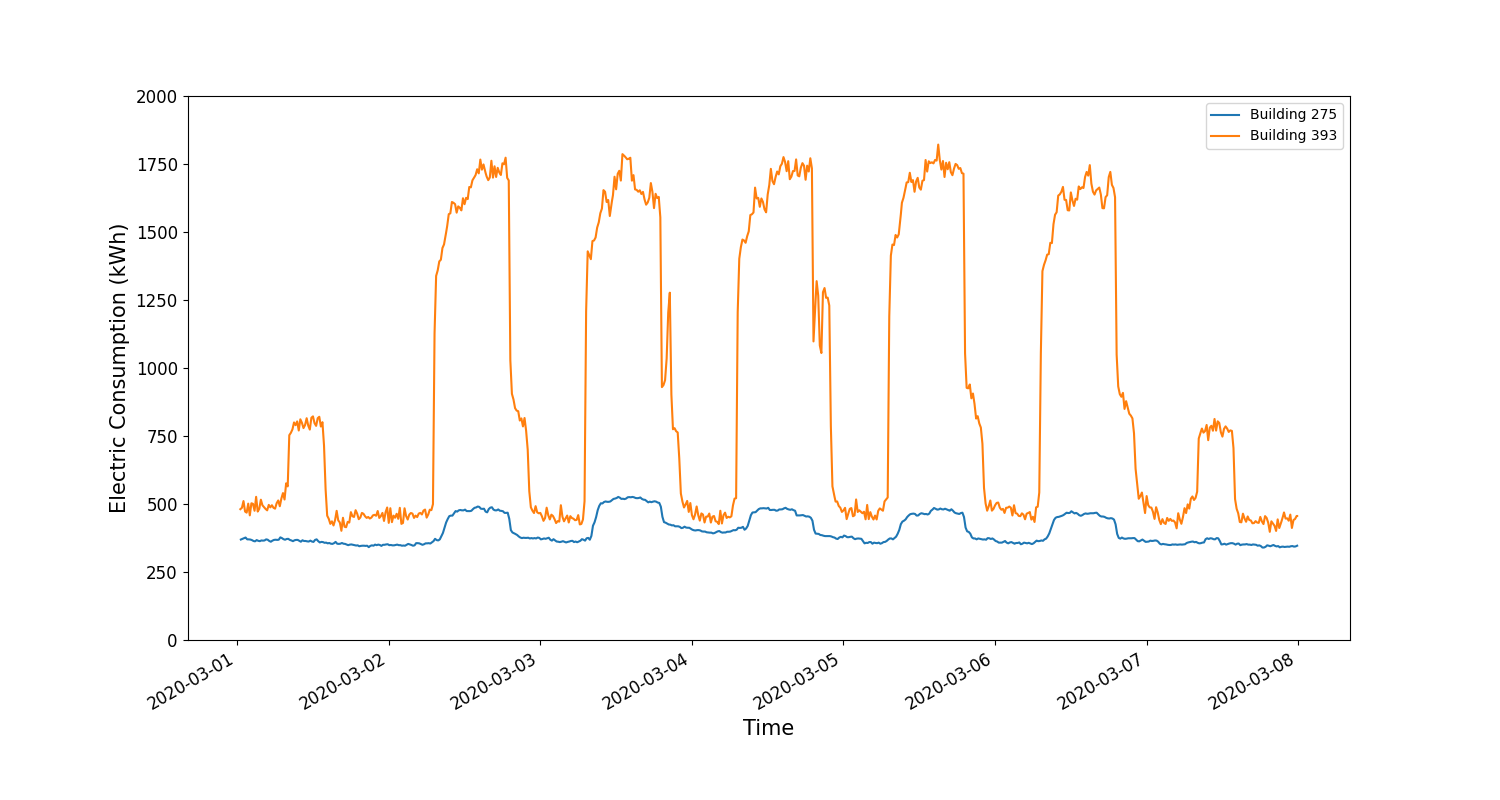
\includegraphics[width=.8\columnwidth]{./images/275v393_Turndown.png}

If 275 was able to achieve the same turndown as 393, which is not extremely unusual in the commercial office group, it would reduce its total energy use by an estimated 36\%. Extrapolating from the 6 months of available energy usage data, this would result in savings of 5,000,000 kWh or nearly \$750,000 of reduced consumption charges per year, based on a 15-cent per kWh cost.

\subsection{Building 390}

Building 390 has a large occupied duration factor, at 0.798. This is a food and beverage facility, and an investigation of the energy consumption usage shows that the consumption is high from roughly 4AM to midnight each evening.

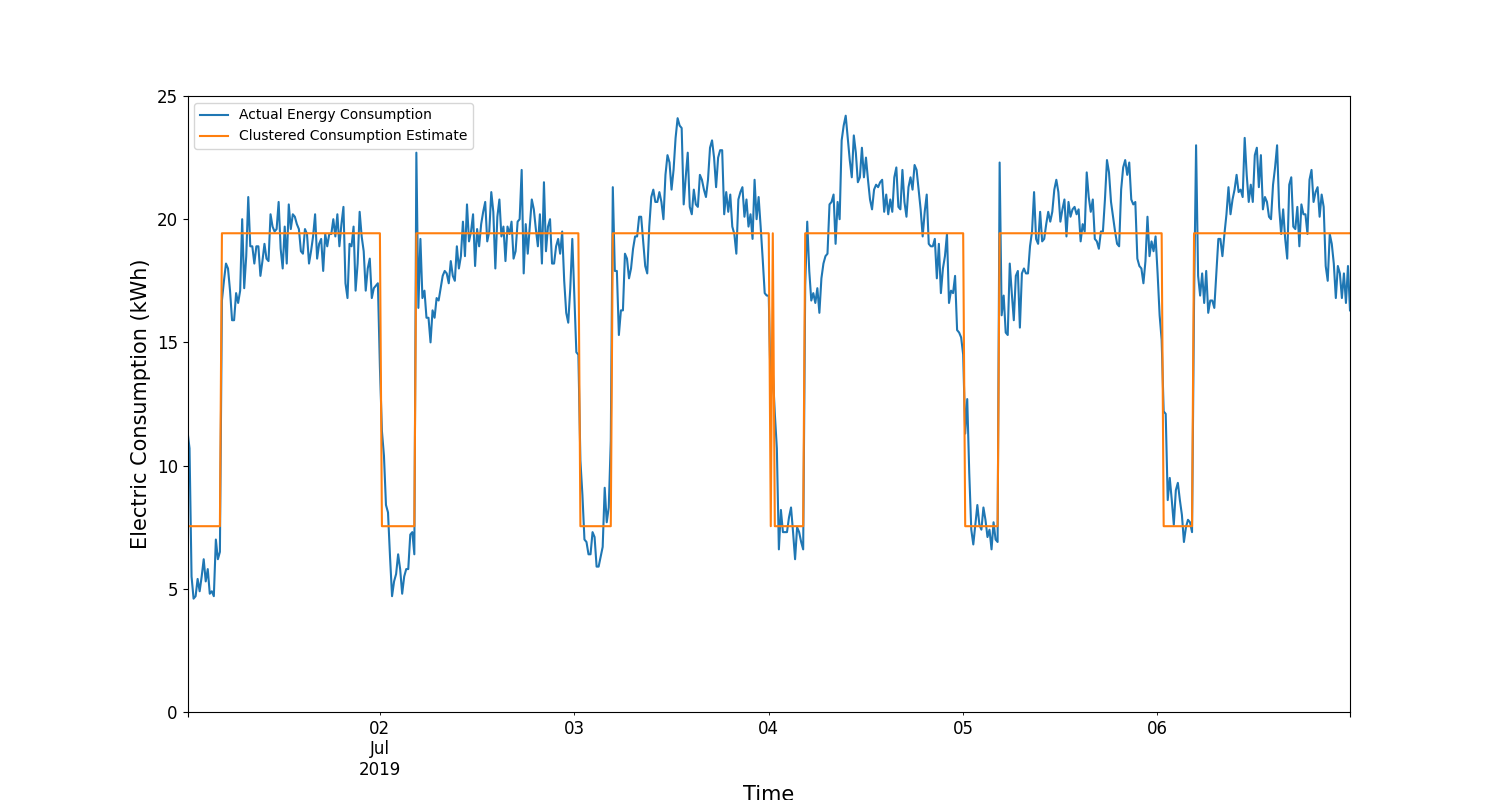
\includegraphics[width=.8\columnwidth]{./images/390_Duration.png}

There are certainly food and beverage facilities that keep these hours, as staff prep in the morning and clean up at night. However a quick investigation could determine if the energy usage profile reflects actual occupancy schedules. If not, and the building could be run in an unoccupied mode even just 2 additional hours each day, that would save nearly 5\% of this building's total energy consumption.

\section{Future Expansion}

As the RTEM dataset grows, these weekly KPIs can be automatically computed on new data. In fact, running the analysis on the entire current RTEM dataset only takes a few minutes on commodity hardware.

The automation of this process suffers from incomplete data modeling of electrical metering within the RTEM dataset. For example, given a site with multiple electric consumption readings, it is not denoted whether a specific reading is a subset of another or fully separate. Top level consumption readings are not differentiated from low-level submeters. Due to this, the final point list used within the analysis was manually reviewed and revised to determine which points (or collection of points) represented each building as a whole. Project Haystack models metering trees using the submeterOf\footnote{https://project-haystack.org/doc/lib-phIoT/submeterOf} tag, and denotes top-level metering using a meterScope\footnote{https://project-haystack.org/doc/lib-phIoT/meterScope} tag. Brick Schema models building-level meters with a Building\_Meter\footnote{https://brickschema.org/ontology/1.2/classes/Building\_Meter} class. Integration of these ideas into the RTEM dataset would improve future automation efforts.

\section{Additional Applications}

The clustering approach shown in this document is not specific to total-building electric energy use. Rather, it could potentially be applied in very similar ways to:
\begin{enumerate}
\item{Other building-level utilities: Total building gas, chilled water, or steam use}
\item{Submetering: Zone or tenant-level unoccuiped setback analysis and tracking}
\item{Downstream occupancy effectiveness metrics: Zone air temperature setpoints, VAV discharge airflow}
\end{enumerate}

\section{Conclusion}

This document presents a strategy for analyzing the effectiveness and prevalence of unoccupied setbacks by using a clustering algorithm on a historical whole-building consumption record. It outlines the KPIs that can be calculated from this record, and demonstrates how they can be used on real-world data from the RTEM dataset. Finally, it discussed the feasibility of expanding this analysis as the RTEM dataset grows.

Energy conservation is the most cost-effective means of decarbonization. Of course, investments must be made in switching fossil fuel-based technologies to clean energy, and expanding renewable energy production. However, in the meantime, we also need to make sure that our existing infrastructure is working as efficiently and effectively as possible. Poor unoccupied operation is the largest opportunity in most buildings that does not require a capital investment. We ought to make sure it is working well and continues to do so.


\end{document}